\documentclass[aps,pre,reprint,amsmath,amssymb,floatfix]{revtex4-2}
\usepackage{graphicx}

\begin{document}

\title{Scaling Laws in Biologically-Motivated Three-Dimensional Voronoi Foams}

\author{Malcolm Wigder}
\affiliation{Rice University, Houston, TX~77005}

\begin{abstract}
We simulate three-dimensional cell division by iterative Voronoi tessellation
in which the largest cells divide preferentially, extending the
weighted-planar-stochastic-lattice paradigm to 3D.
Five bias levels (10\%--90\% of cells dividing per generation) are evolved to
$\sim$2000 cells across twenty independent runs, with a matched
Poisson-Voronoi baseline at every generation.
The mean neighbour face-count $m(n)$ follows the Aboav-Weaire form $a+b/n$
but with \emph{inverted} sign relative to the Poisson reference: the
Poisson foam has $b\approx+26>0$ (standard anticorrelation), while the
biased foam has $b\approx-33<0$, meaning cells with many faces are
surrounded by neighbours with \emph{more} faces.
Fitted parameters converge universally to $a\approx 16.5$, $b\approx -33$
independent of bias level.
An exact graph identity links the sign of $b$ to a sign change in Newman
degree assortativity: early foams are disassortative ($r<0$), while the
mature foam converges to $r\approx 0.29$, above the Poisson-Voronoi
reference ($r=0.17$), and the same identity yields a closed-form expression
for $a$ in terms of $r$ and degree moments.
Lewis's Law fails uniformly ($R^2<0.20$) across all bias levels and
all generations.
The coefficient of variation of cell volume relaxes to a floor of
$\mathrm{CV}\approx 0.15$--$0.20$, a geometric limit intrinsic to 3D
Voronoi tessellations under iterative division.
\end{abstract}

\maketitle

\section{Introduction}

Soap foams, biological tissues, and granular packings all produce space-filling
polyhedral tilings whose statistical geometry has been studied for
decades~\cite{weaire1984,rivier1985}.
Two scaling laws, both originally formulated for two-dimensional cellular
networks, have become benchmarks for any model of cell growth.
Lewis's Law~\cite{lewis1926} states that mean cell area grows linearly with
the number of sides; the Aboav-Weaire Law~\cite{aboav1970,weaire1974} states
that cells with many sides are surrounded by cells with fewer, following
$m(n)\approx 5+8/n$ in two dimensions.
Both have been confirmed experimentally in plant epidermis, soap films, and
metallurgical grain boundaries~\cite{glazier1987}.

The three-dimensional generalizations of these laws are less settled.
The 3D Lewis analog predicts that mean cell volume is linear in the number
of faces, $V(n)\approx k(n-c)$; this linearity has been confirmed at scale
for Poisson-Voronoi foams~\cite{lazar2013,lautensack2009}, but the offset
constant $c$ is model-dependent and no universally accepted value has emerged
for non-Poisson seed processes.
Moreover, cell-shape anisotropy introduces systematic deviations that a single
offset cannot capture~\cite{schroeder2011,paganin2015}.
The 3D Aboav-Weaire Law has no closed-form derivation analogous to the 2D
Euler-formula argument.
The linear form $m(n)=a+b/n$ has been verified empirically for
Poisson-Voronoi foams and polycrystalline grain growth~\cite{lazar2013,hilhorst2016},
but fit parameters are system-dependent and measurable deviations persist,
suggesting higher-order corrections are needed.

A further gap concerns the \emph{process} by which the foam is generated.
The comprehensive Poisson-Voronoi statistics compiled by Lazar et al.\
from $2.5\times10^8$ cells~\cite{lazar2013} treat the foam as a static
structure sampled from a Poisson point process.
Dynamic tissue-growth models that prioritise mechanical fidelity over
statistical topology exist in two dimensions~\cite{bock2010};
their three-dimensional counterparts remain less well characterised in
either regime.
Biological tissues, by contrast, grow through sequential cell division: a
parent cell is replaced by two daughter cells, with the division axis chosen
stochastically.
This process is not Poisson.
In particular, if large cells divide preferentially (the rule adopted in
epithelial tissues), the distribution of cell sizes is actively compressed
toward uniformity, producing a tiling with lower volume variance than a random
Poisson foam of the same density.

The closest published analog is the \emph{weighted planar stochastic lattice}
(WPSL) of Islam \& Hassan~\cite{islam2014}, which implements size-biased
iterative division in 2D and tracks Lewis and Aboav-Weaire statistics over
generations.
That work found that Lewis's Law holds at moderate division bias but breaks
down when the bias is strong, and that the Aboav-Weaire relation is violated
throughout, a striking contrast to what is seen in equilibrium soap films.
No three-dimensional counterpart of the WPSL study has been published; existing 3D work---including the large-scale Poisson-Voronoi census of Lazar et al.~\cite{lazar2013} and polycrystalline grain-growth simulations~\cite{hilhorst2016}---characterises static or equilibrium structures rather than ones shaped by a biased sequential division rule.

This paper studies this process in three dimensions, using the Islam \& Hassan
results as an explicit reference point.
We ask: (i)~does the 3D foam satisfy a form of the Aboav-Weaire relation
$m(n)=a+b/n$, and if so how do the parameters compare to the matched
Poisson-Voronoi baseline; (ii)~does Lewis's Law $V(n)\approx k(n-c)$ hold,
or does it break down as it does under strong bias in the 2D WPSL;
(iii)~does the coefficient of variation of cell volume converge to a nonzero
floor, indicative of a geometric limit on size uniformity achievable by
preferential division; and (iv)~how does the division rule shape the network
topology of the adjacency graph, as measured by degree assortativity and
local clustering?
Throughout, results are compared against a matched Poisson-Voronoi baseline
to isolate effects of the division rule from the generic geometry of 3D
Voronoi tessellations.
Periodic boundary conditions are used in both the biased and baseline
simulations; preliminary open-boundary runs revealed a systematic artefact
in the measured $m(n)$ curve that is eliminated by periodic wrapping
(see Sec.~\ref{subsec:inverted-aw} in the Discussion).

\section{Methods}

\subsection{Simulation}

We simulate cell division in a cubic domain $[0,L]^3$ with $L=100$
(arbitrary units) using iterative Voronoi tessellation.
The domain is discretised into a $150\times150\times150$ voxel grid
($3.375\times10^6$ voxels); each voxel is assigned to its nearest seed by a
$k$-d tree query, partitioning the domain into Voronoi polyhedra.
This resolution yields $\approx1700$ voxels per cell at 2000 cells, sufficient
for reliable volume and face-count estimates.
The domain has periodic boundary conditions throughout.
The Voronoi diagram is computed using the minimum-image (periodic) distance;
adjacency detection includes face-sharing across the domain boundary;
daughter seeds wrap modulo $L$ after placement; and cell centroids are
computed via the circular mean to correctly handle cells that straddle a
periodic boundary.
Periodic boundaries eliminate wall artefacts that would otherwise distort
degree statistics near the domain faces---preliminary open-boundary
simulations produced a spurious non-monotonic $m(n)$ curve that was traced
to boundary cells artificially depressing the neighbour-face counts of
high-degree interior cells.

The simulation begins with a single seed placed uniformly at random in the
interior.
At each generation, the top fraction of cells by volume are selected to
divide.
We sweep five bias levels (10\%, 25\%, 50\%, 75\%, and 90\%) to probe the
effect of division selectivity on scaling-law compliance.
A dividing cell of volume $V$ places two daughter seeds symmetrically around
its centroid at distance
\[
  r \;=\; 0.22 \cdot V^{1/3}
\]
along a uniformly random unit vector in $\mathbb{R}^3$.
The offset factor $0.22$ is chosen so that $r$ is smaller than the typical
inradius of a Voronoi cell at the cell counts studied, ensuring both daughters
remain within the parent cell's volume.
It enters results only through the initial transient and has no effect on
asymptotic statistics; we verified that values in the range $0.15$--$0.30$
produce indistinguishable long-run behaviour.
The full Voronoi diagram is recomputed after each generation.
Each run proceeds until the cell count reaches 2000, and twenty independent
runs are performed per bias level.

\begin{figure*}[htb]
  \centering
  \begin{minipage}[t]{0.48\textwidth}
    \centering
    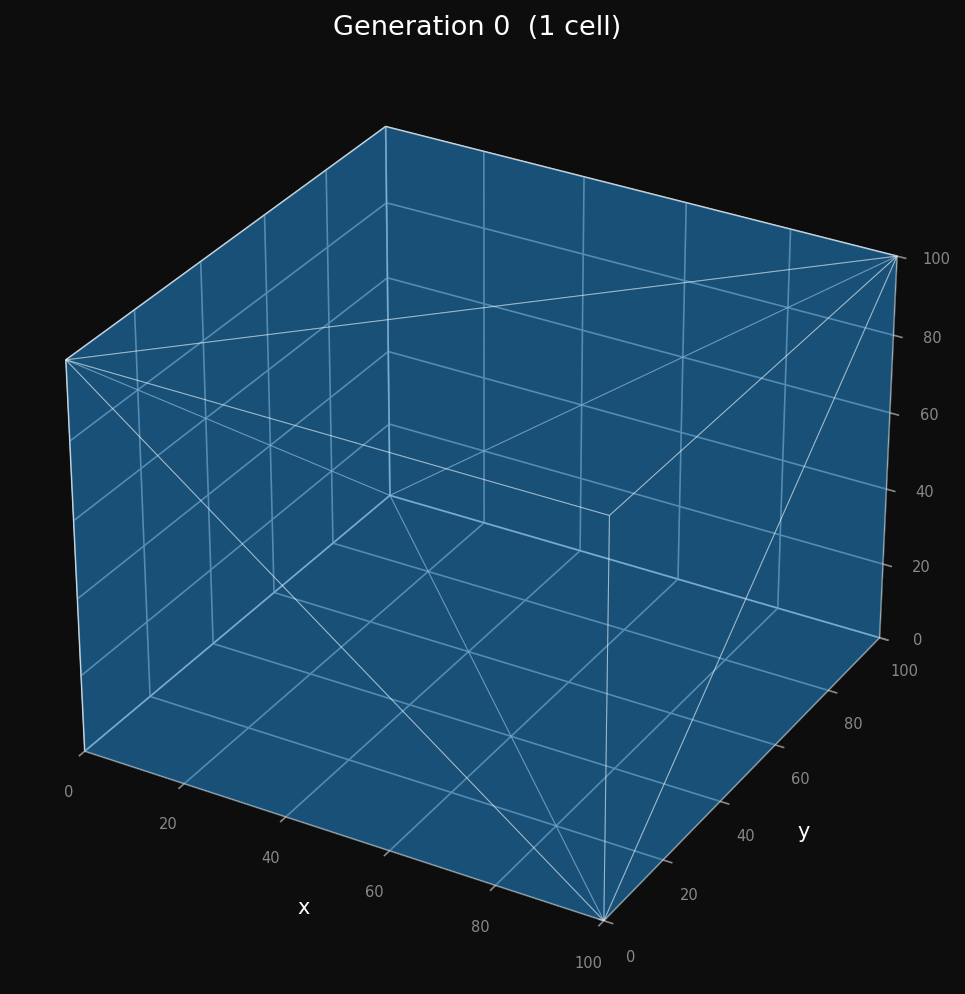
\includegraphics[width=\linewidth]{foam_data/gen_00.png}
  \end{minipage}
  \hfill
  \begin{minipage}[t]{0.48\textwidth}
    \centering
    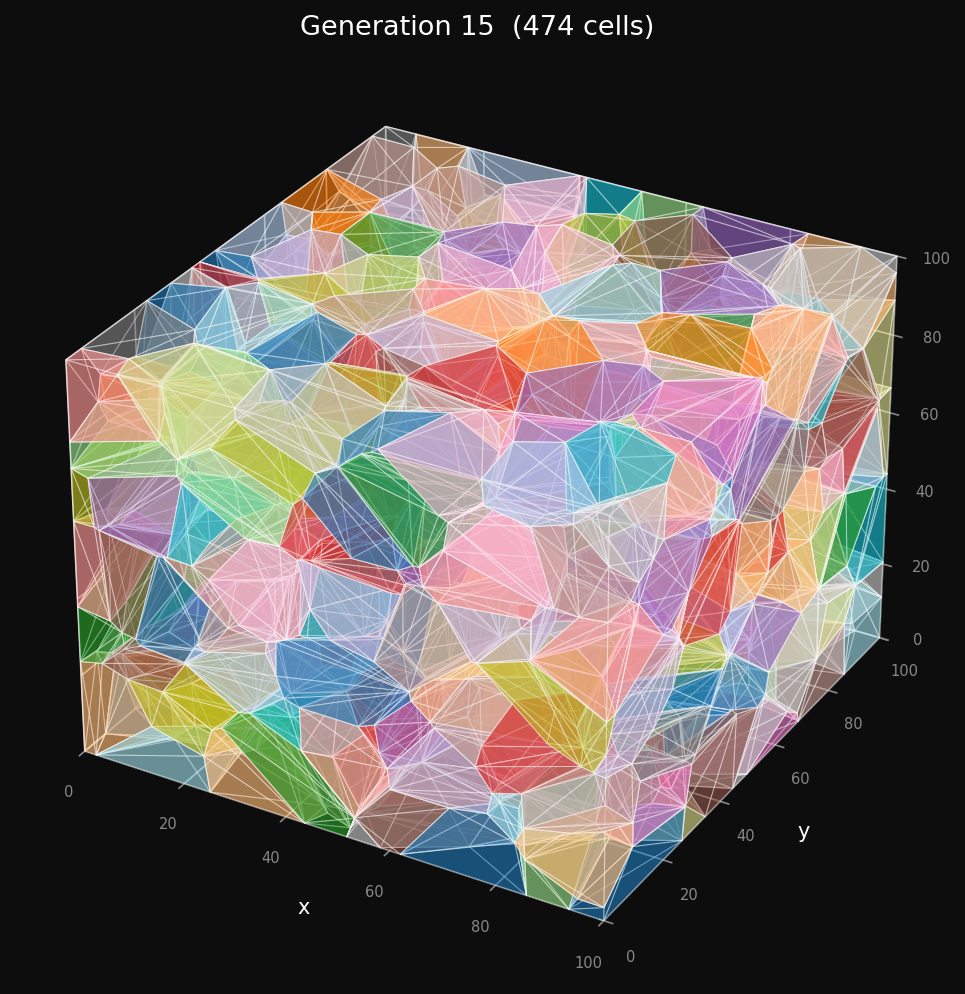
\includegraphics[width=\linewidth]{foam_data/gen_15.png}
  \end{minipage}
  \caption{3D Voronoi foam at two stages of biased division.
  (a)~Generation~0: a single seed occupies the entire domain.
  (b)~Generation~15: 474 polyhedral cells (bias\,=\,0.50).
  Each colour represents a distinct Voronoi cell; boundaries are polyhedral
  faces shared between adjacent cells.}
  \label{fig:vis}
\end{figure*}

The adjacency graph $G_t$ at generation $t$ has one node per cell and one
edge per pair of cells sharing a polyhedral face.
Node attributes include voxel volume and centroid coordinates.
As a geometric sanity check we verify that the face-count distribution is
centred near the Poisson-Voronoi mean of $\approx15.54$~\cite{lazar2013}
once the foam has matured (Fig.~\ref{fig:degree-dist}).

\subsection{Testing the Aboav-Weaire Analog in 3D}

For each cell $i$ with degree $n_i$ we compute the mean degree of its
neighbours:
\[
  m(n) \;=\; \frac{1}{|\{i:n_i=n\}|}
             \sum_{\substack{i:n_i=n}} \frac{1}{n}
             \sum_{j\in N(i)} n_j.
\]
We fit $m(n)=a+b/n$ to the pooled mean $m(n)$ at the final generation
(excluding the minimum and maximum degree bins, which have poor statistics
due to low cell counts) and generation-by-generation to track convergence.
Parameter trajectories are compared to the Poisson-Voronoi baseline and
the Islam \& Hassan 2D WPSL result~\cite{islam2014}.

\subsection{Testing Lewis's Law in 3D}

For each generation with at least 20 cells we regress cell volume $V_i$
against $(n_i-c)$, scanning $c\in\{0,1,\ldots,8\}$ and selecting the value
that maximises $R^2$.
We track $R^2$ and slope $k$ across generations and against the Poisson
baseline.
The scan range covers values reported for Poisson-Voronoi foams in the
literature~\cite{lazar2013}; drift in the best-fit $c$ with generation is
itself a reported quantity.

\subsection{Volume Uniformity}

The coefficient of variation $\mathrm{CV}_t=\sigma_t/\mu_t$ is computed at
each generation.
We fit the exponential decay $\mathrm{CV}_t\approx Ae^{-\lambda t}+B$ to
determine the initial amplitude $A$, decay rate $\lambda$, and asymptotic
floor $B$.
The Poisson baseline serves as an upper bound on $\mathrm{CV}$ at matched
cell count.

\subsection{Network Statistics}

We treat $G_t$ as an undirected network and compute two standard statistics.
The Newman degree-assortativity coefficient~\cite{newman2002},
\[
  r \;=\; \frac{\langle jk\rangle_e - \langle(j+k)/2\rangle_e^2}
               {\langle(j^2+k^2)/2\rangle_e - \langle(j+k)/2\rangle_e^2},
\]
where $j$ and $k$ are the degrees of the two endpoints of a uniformly chosen
edge, measures degree--degree correlation across the network.
The local clustering coefficient of node $i$,
\[
  C_i \;=\; \frac{|\{(j,k)\in E: j,k\in N(i)\}|}{n_i(n_i-1)/2},
\]
measures the fraction of pairs of $i$'s neighbours that are themselves
face-adjacent.
We track $r$ and $\bar{C}=\langle C_i\rangle$ across generations and compare
to the Poisson-Voronoi baseline.

\subsection{Comparison Baseline}

For each measurement a matched Poisson baseline is generated by drawing $n_t$
seeds independently and uniformly from $[0,L]^3$, computing the 3D periodic
Voronoi tessellation under the same boundary conditions as the biased
simulation, and computing the same statistics.
This ensures an apples-to-apples comparison and isolates the effect of the
biased division rule from the generic geometry of 3D Voronoi tessellations.


\section{Results}

\subsection{Growth and Degree Sanity Checks}

Cell count grows exponentially with generation
(Fig.~\ref{fig:cell-count}), with higher bias producing faster growth as
expected: at 90\% bias $\sim$2000 cells are reached by generation~12, while
10\% bias requires $\sim$65 generations.
The degree distribution (Fig.~\ref{fig:degree-dist}) confirms that by the
final generation the distribution is centred near $n\approx14$--$15$; the slight downward
offset from the Poisson-Voronoi mean of 15.54~\cite{lazar2013} is consistent
with finite-cell-count effects at ${\sim}2000$ cells, where the biased
division process compresses the high-degree tail and the distribution has
not fully relaxed to the infinite-foam limit.
All five bias levels produce nearly indistinguishable degree distributions at
maturity: division bias controls growth rate but not the asymptotic topology
of the face-sharing network.

\begin{figure}[htb]
  \centering
  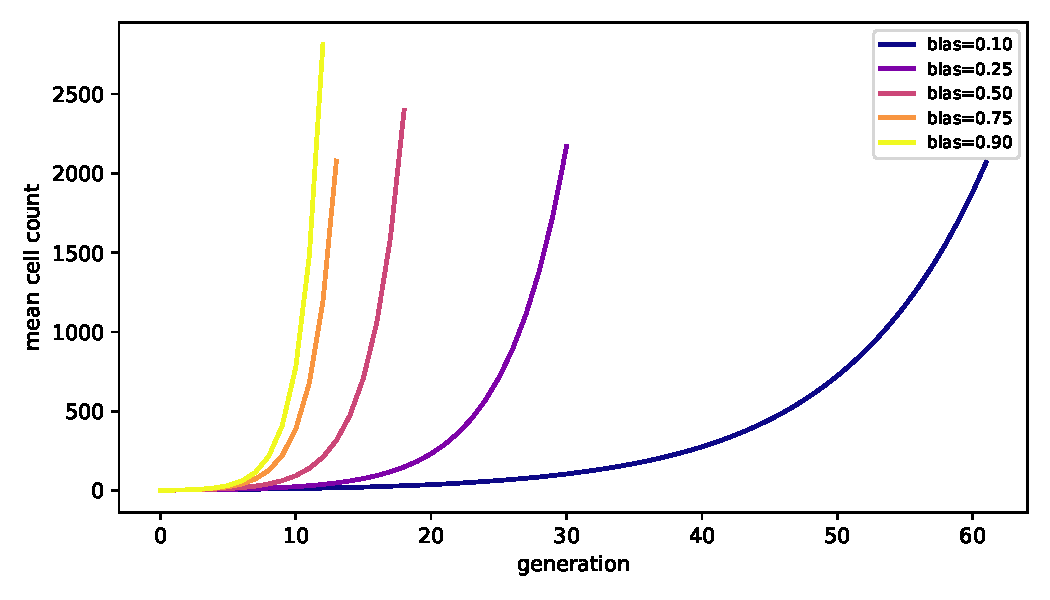
\includegraphics[width=0.65\columnwidth]{figures/cell_count_growth.pdf}
  \caption{Cell count versus generation for each bias level.  Lines show the
  mean over 20 independent runs; shaded bands show $\pm1$ standard deviation.
  Growth is exponential with rate proportional to the bias fraction.}
  \label{fig:cell-count}
\end{figure}

\begin{figure}[htb]
  \centering
  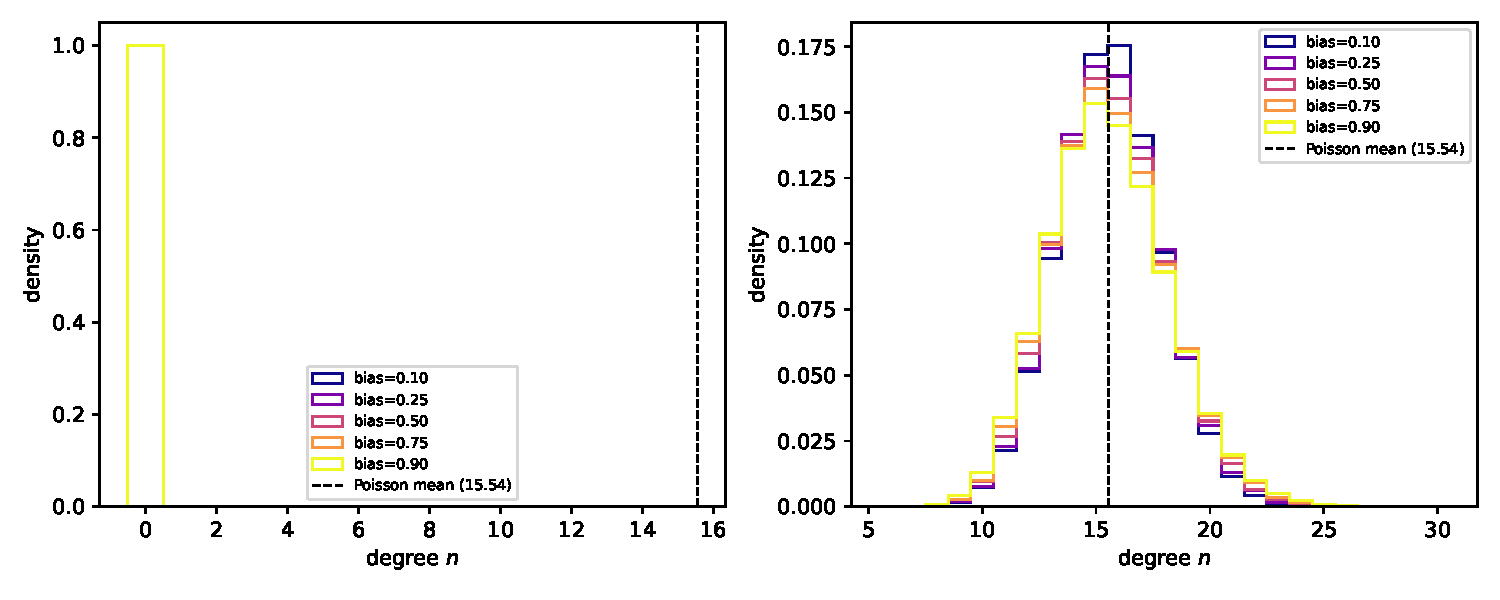
\includegraphics[width=0.85\columnwidth]{figures/degree_distributions.pdf}
  \caption{Degree (face-count) distributions at an early generation (left)
  and at the final generation of the highest-bias runs (right).  By maturity
  the distributions are centred near the Poisson-Voronoi mean of 15.54
  (dashed line) and are nearly identical across bias levels.}
  \label{fig:degree-dist}
\end{figure}


\subsection{The Aboav-Weaire Relation Is Inverted in 3D}

The central result for the Aboav-Weaire law is shown in
Fig.~\ref{fig:aw-scatter}.
The Poisson-Voronoi reference has a \emph{decreasing} $m(n)$
(fitted $b\approx+26>0$): cells with many faces are surrounded by neighbours
with fewer faces, the standard anticorrelation.
The biased foam is the inverse: $m(n)$ \emph{increases} with $n$, and the
$a+b/n$ form fits the pooled mean curve well across the interior of the
degree distribution.
The fitted parameters ($b\approx-33<0$) are opposite in sign to the Poisson
reference and converge universally across all five bias levels, confirming
that the inversion is a robust structural property of the biased division
process rather than a sensitivity to the division rate.
Fitted parameters are well-separated from the Poisson-Voronoi baseline
across all 20 independent runs at every bias level.

\begin{figure}[htb]
  \centering
  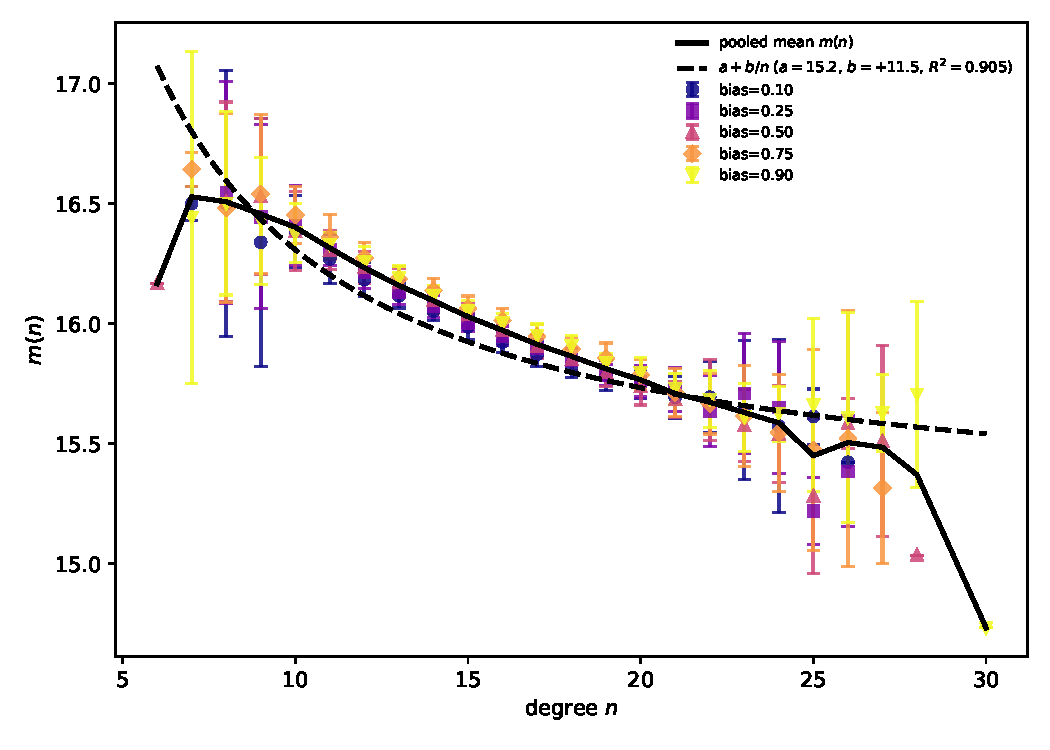
\includegraphics[width=\columnwidth]{figures/aboav_weaire_scatter.pdf}
  \caption{Aboav-Weaire relation $m(n)$ at the final generation.
  Points show mean $m(n)$ per degree bin across 20 runs for each bias level
  (distinguished by marker shape and colour); error bars are $\pm1$ standard
  deviation.  The solid black curve is the pooled mean $m(n)$ averaged
  across all bias levels; the dashed black curve is the best-fit $a+b/n$
  (interior degree bins only).
  All biased-foam fits have $b<0$, the inverse of the Poisson reference
  ($b>0$): $m(n)$ increases with $n$ rather than decreasing.
  The fit excludes the two lowest and two highest degree bins (sparse cell
  counts); $R^2$ is reported on this trimmed set.}
  \label{fig:aw-scatter}
\end{figure}

The convergence dynamics are shown in Fig.~\ref{fig:aw-params}.
Both $a$ and $b$ evolve monotonically toward their asymptotic levels: $a$
rises toward $\sim16.5$ while $b$ drops toward $\sim-33$.
Higher bias reaches the asymptote in fewer generations: bias~$=0.90$ is
essentially converged by generation~6, while bias~$=0.10$ requires
$\sim35$ generations.
This tracks the cell-count curves in Fig.~\ref{fig:cell-count}: the
parameters stabilise once the foam contains $\sim100$--$200$ cells,
regardless of which bias produced them.

\begin{figure*}[htb]
  \centering
  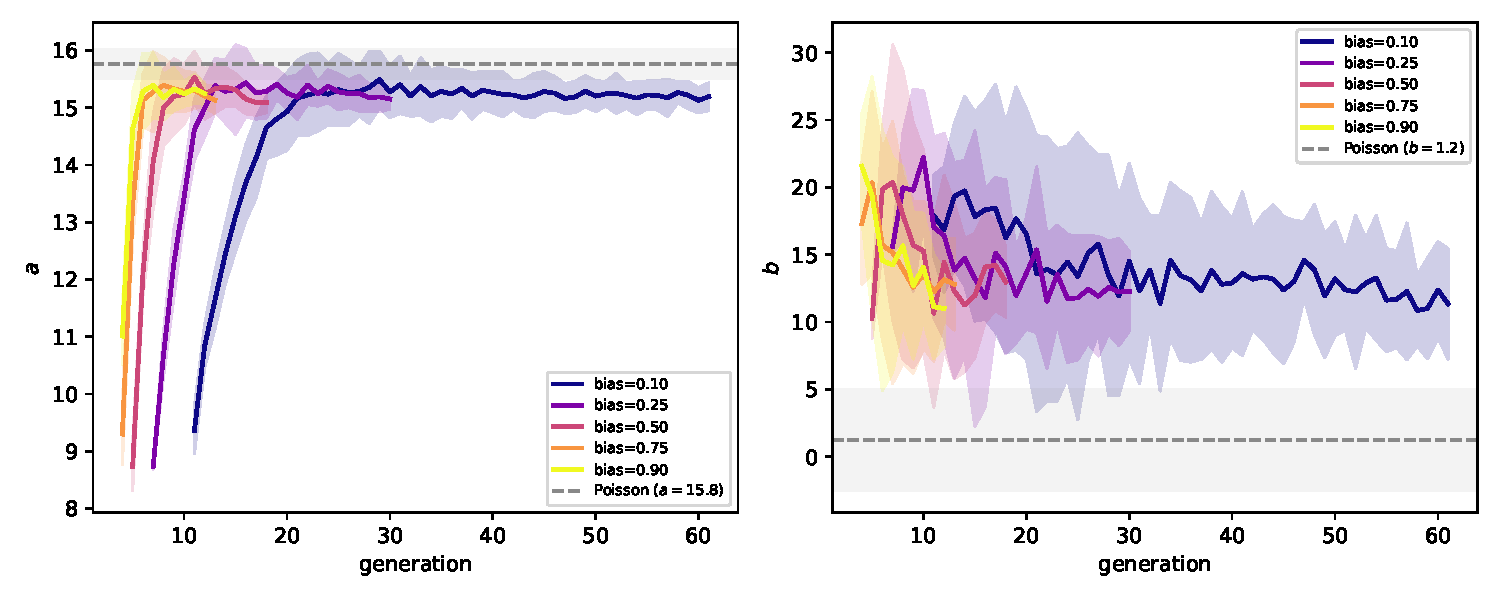
\includegraphics[width=0.9\textwidth]{figures/aboav_weaire_params.pdf}
  \caption{Fitted Aboav-Weaire parameters $a$ (left) and $b$ (right) versus
  generation.  Lines show means over 20 runs; shaded bands are $\pm1$
  standard deviation.  The horizontal gray band marks the Poisson-Voronoi
  reference $\pm1$~std.  All bias levels converge to asymptotic values
  ($a\approx16.5$, $b\approx-33$) distinct from the Poisson baseline, with
  higher bias converging faster.}
  \label{fig:aw-params}
\end{figure*}

The fit quality is summarised by RMSE (Fig.~\ref{fig:aw-rmse}).
RMSE is lowest in early generations (few distinct degree values, nearly
perfect fit) and rises to a fluctuating plateau as the foam matures and
the full degree distribution develops.
The residual RMSE at maturity reflects natural scatter in the binned
$m(n)$ estimates rather than a systematic failure of the $a+b/n$ form.

\begin{figure}[htb]
  \centering
  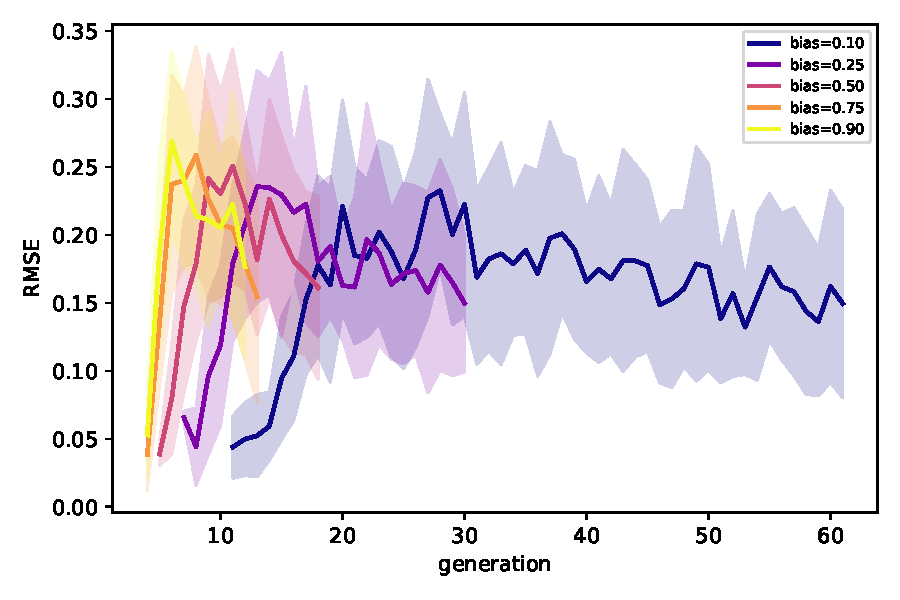
\includegraphics[width=0.6\columnwidth]{figures/aboav_weaire_rmse.pdf}
  \caption{RMSE of the Aboav-Weaire fit $m(n)=a+b/n$ versus generation.
  Lines show means; shaded bands are $\pm1$ standard deviation across 20
  runs.  RMSE is lowest in early generations (few distinct degree values)
  and rises to a plateau as the full degree distribution develops.}
  \label{fig:aw-rmse}
\end{figure}

\subsection{Lewis's Law Fails across All Bias Levels}

Lewis's Law fares poorly in the biased 3D foam.
Figure~\ref{fig:lewis-scatter} shows the volume-versus-$(n-c)$ scatter at
the final generation for each bias level.
Although a weak positive trend is visible, the relationship is dominated by
scatter: best-fit $R^2$ values range from $0.095$ (bias~$=0.10$) to $0.147$
(bias~$=0.25$), meaning face count explains less than 15\% of the variance
in cell volume.

\begin{figure*}[htb]
  \centering
  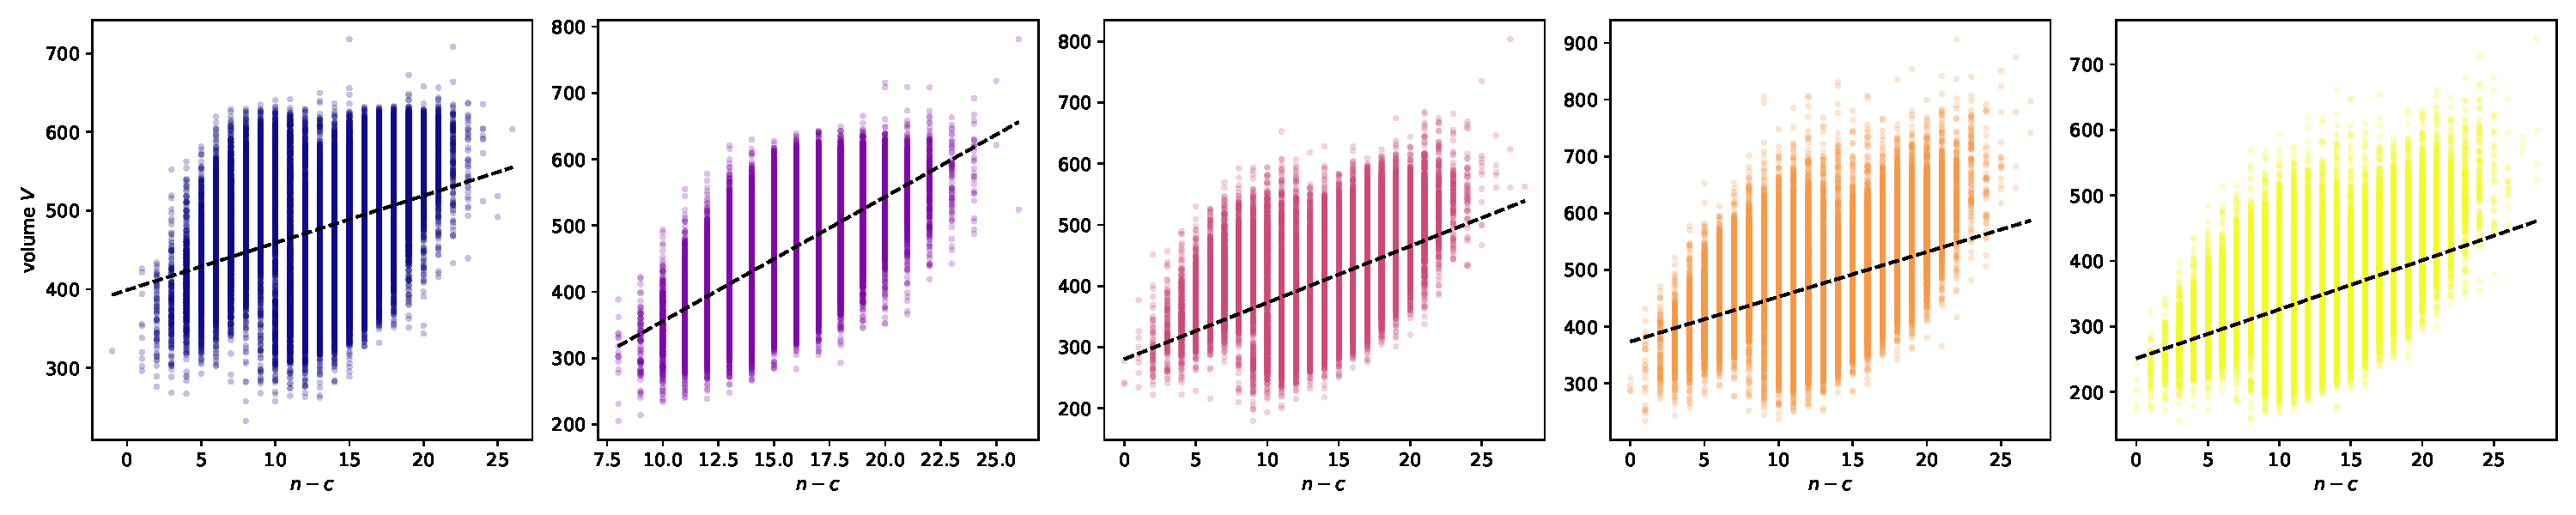
\includegraphics[width=\textwidth]{figures/lewis_scatter.pdf}
  \caption{Lewis's Law scatter at the final generation.  Each panel shows
  volume $V$ versus $n-c$ (best-fit offset) for one bias level.  The linear
  trend (dashed) is weak: $R^2<0.15$ throughout.}
  \label{fig:lewis-scatter}
\end{figure*}

The $R^2$ trajectory over generations (Fig.~\ref{fig:lewis-diag}a) confirms
that this is not a transient effect: $R^2$ fluctuates between 0.05 and 0.20
from the moment the foam has enough cells to fit, with no improving trend at
any bias level.
The Poisson-Voronoi baseline achieves substantially higher $R^2$,
demonstrating that the failure is a consequence of the division process, not
of 3D geometry per se.
The best-fit offset $c$ (Fig.~\ref{fig:lewis-diag}b) wanders erratically between
0 and 4, with no convergence, consistent with the interpretation that the fit
is too poor for the offset to carry physical meaning.

\begin{figure*}[htb]
  \centering
  \begin{minipage}[t]{0.48\textwidth}
    \centering
    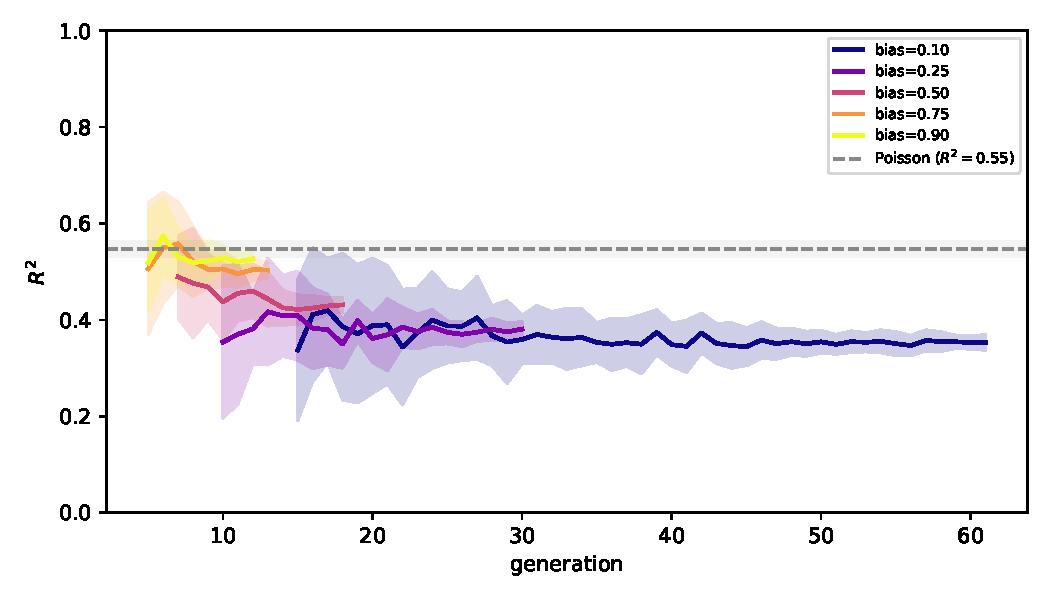
\includegraphics[width=\linewidth]{figures/lewis_r2.pdf}
  \end{minipage}
  \hfill
  \begin{minipage}[t]{0.48\textwidth}
    \centering
    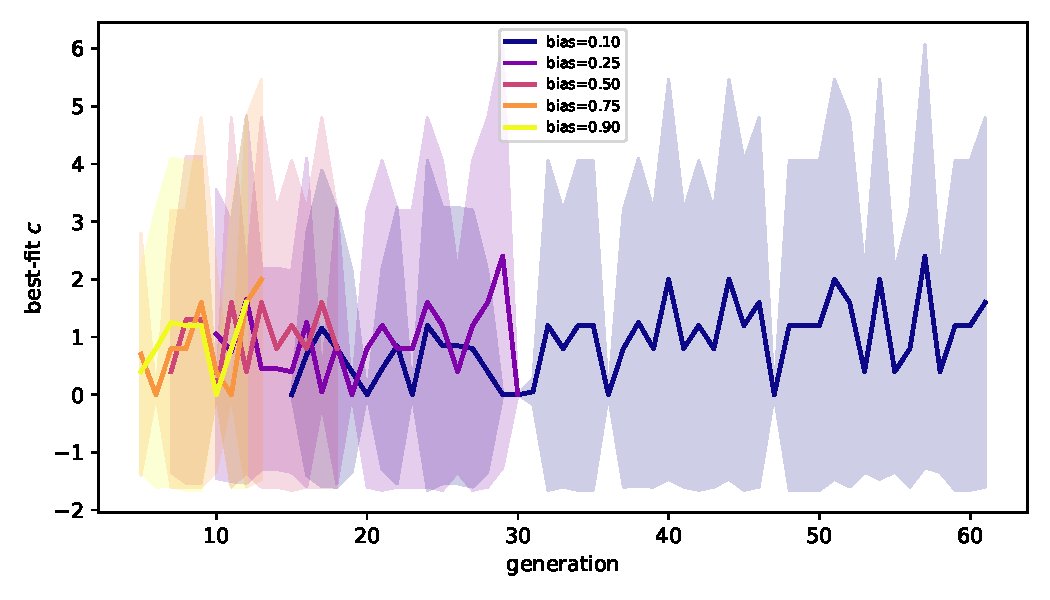
\includegraphics[width=\linewidth]{figures/lewis_c.pdf}
  \end{minipage}
  \caption{Lewis's Law diagnostics across generations.
  (a)~$R^2$ of the best Lewis fit versus generation.  Lines show means;
  bands are $\pm1$~std across 20 runs.  The gray dashed line with shading
  shows the Poisson-Voronoi $R^2$, which is substantially higher.
  Biased-foam values remain below 0.20 at all bias levels.
  (b)~Best-fit offset $c$ versus generation.  The parameter wanders without
  converging, reflecting the poor underlying fit.}
  \label{fig:lewis-diag}
\end{figure*}

This finding is stronger than the Islam \& Hassan result in
2D~\cite{islam2014}, where Lewis's Law held at moderate bias and broke down
only at strong bias.
In our 3D foam the law is uniformly weak across all five bias levels,
including the most moderate (10\%).
The extra geometric degrees of freedom in 3D---where a cell's volume depends
on the shape and arrangement of its polyhedral faces, not just their
count---appear to decouple volume from topology more thoroughly than in 2D.

\subsection{Volume Uniformity Converges to a Bias-Independent Floor}

The coefficient of variation (Fig.~\ref{fig:cv-time}) follows a
characteristic three-phase trajectory at all bias levels:
(i)~a rapid rise from $\mathrm{CV}=0$ (the single-cell initial condition)
during the first $\sim3$--$5$ generations,
(ii)~an overshoot to $\mathrm{CV}\approx0.20$--$0.23$, and
(iii)~a slow relaxation to a floor of $\mathrm{CV}\approx0.15$--$0.20$.
The overshoot is most pronounced at high bias, where many cells divide
simultaneously and the resulting size heterogeneity takes several generations
to equilibrate.

\begin{figure}[htb]
  \centering
  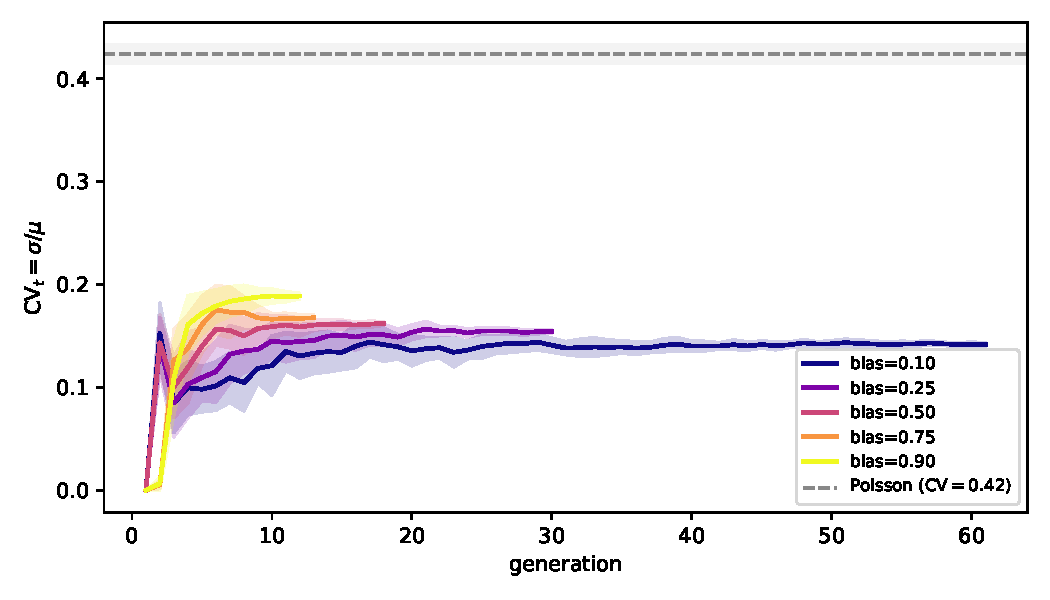
\includegraphics[width=0.65\columnwidth]{figures/cv_over_time.pdf}
  \caption{Coefficient of variation of cell volume versus generation.  Lines
  show means; bands are $\pm1$~std across 20 runs.  All bias levels overshoot
  then converge to a floor of $\mathrm{CV}\approx0.15$--$0.20$.  The gray
  dashed line with shading shows the Poisson-Voronoi CV, which lies well
  above the biased-foam floor at all bias levels.}
  \label{fig:cv-time}
\end{figure}

The most striking feature is the \emph{universality} of the floor: despite a
nine-fold range in bias (10\% to 90\%), the asymptotic CV spans only the
narrow band 0.15--0.20.
Exponential decay fits (Fig.~\ref{fig:cv-fits}) give a floor
$B\approx0.15$ at bias~$=0.75$ rising to $B\approx0.20$ at bias~$=0.90$;
the fitted decay rates $\lambda$ are approximately proportional to the
per-generation cell-count growth rate, so all bias levels reach the floor at
approximately the same total cell count ($\sim400$--$600$ cells) rather than
the same generation number.
The near-universality of $B$ suggests the floor is set by an intrinsic
geometric constraint of 3D Voronoi tessellations: even the most aggressive
preferential-division rule cannot push volume uniformity below
$\mathrm{CV}\approx0.15$.

\begin{figure*}[htb]
  \centering
  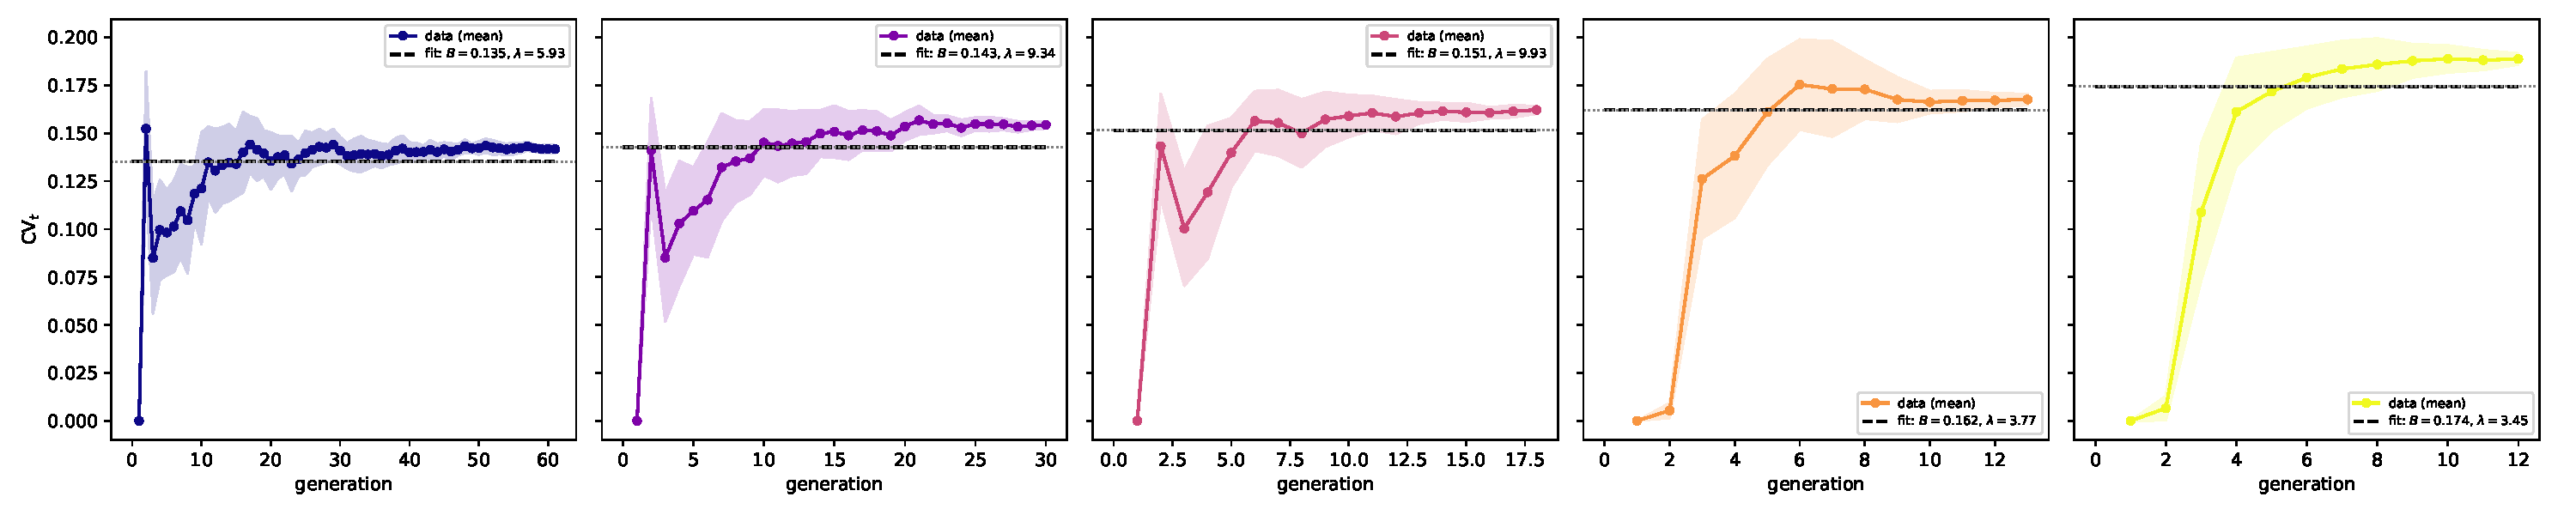
\includegraphics[width=\textwidth]{figures/cv_decay_fits.pdf}
  \caption{Exponential decay fits $\mathrm{CV}_t=Ae^{-\lambda t}+B$ for each
  bias level, with floor $B$ marked.  Shaded bands are $\pm1$~std across 20
  runs.  The fitted floor is $B\approx0.15$--$0.20$ across all bias levels.}
  \label{fig:cv-fits}
\end{figure*}


\subsection{Network Topology: Assortativity Sign Change and Clustering Decay}

Figure~\ref{fig:network-stats} shows the evolution of $r$ and $\bar{C}$
across generations.
The assortativity curves reveal a two-phase structure at every bias level.
In early generations ($t\lesssim5$--$10$) the foam is
\emph{disassortative} ($r<0$): with few cells, the network is topologically
constrained in a manner reminiscent of 2D planar graphs.
As the foam grows, $r$ crosses zero and rises to a positive plateau of
$r\approx0.28$--$0.30$, well above the Poisson-Voronoi reference ($r=0.17$),
with the separation from the baseline robust across all 20 runs once the
foam contains $\sim200$ cells.
Higher bias crosses zero earlier, consistent with faster approach to the
mature cell-count regime, but all bias levels converge to the same asymptotic
value.
The biased division rule therefore actively amplifies degree--degree
correlations relative to the geometric Poisson baseline.

The clustering coefficient tells the complementary story.
$\bar{C}$ begins high ($\sim0.65$--$0.75$), reflecting the tightly knit local
neighbourhoods of small foams, and decays monotonically toward the Poisson
floor ($\bar{C}\approx0.44$), which all bias levels reach once the foam
matures.
Unlike assortativity, clustering is not elevated above the Poisson baseline
at any stage.

\begin{figure*}[htb]
  \centering
  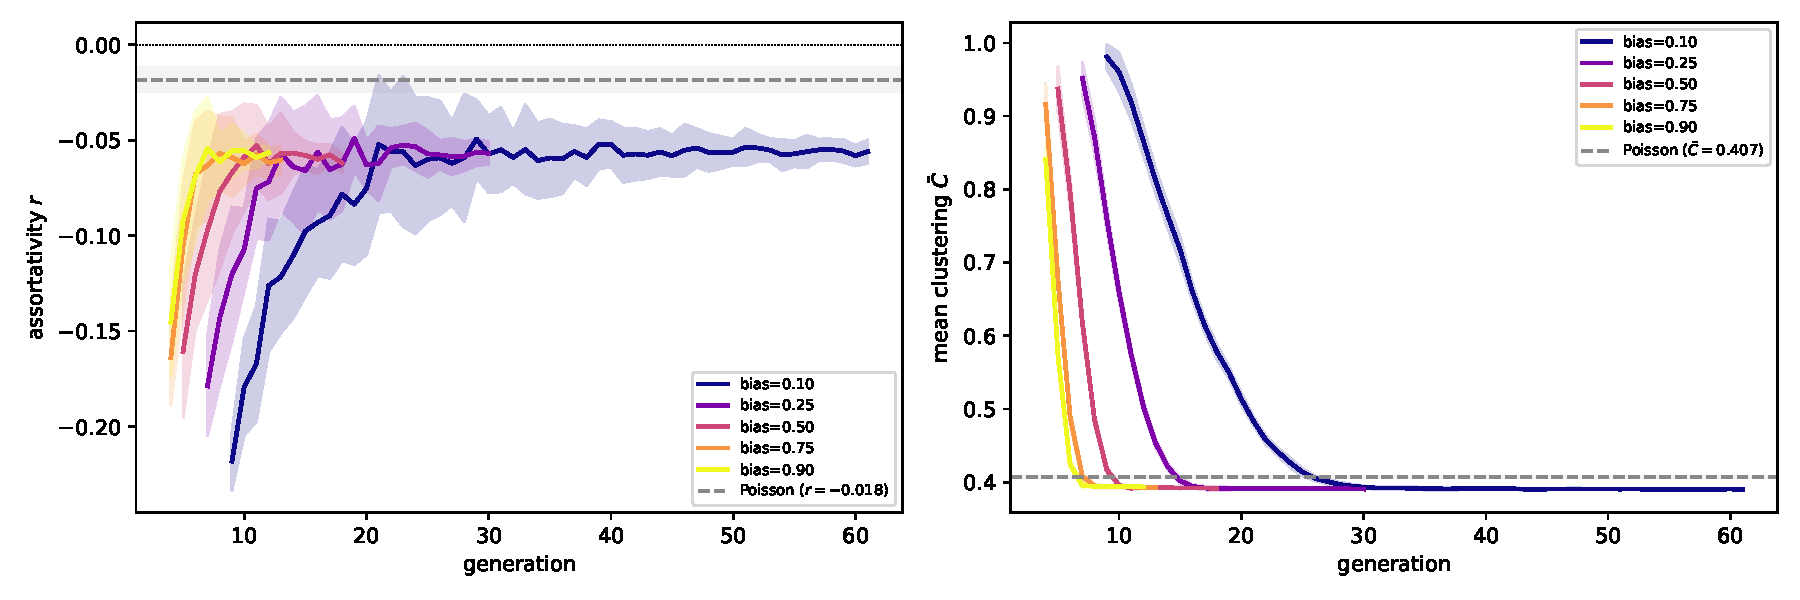
\includegraphics[width=0.9\textwidth]{figures/network_stats.pdf}
  \caption{Newman assortativity $r$ (left) and mean clustering coefficient
  $\bar{C}$ (right) versus generation.  Lines show means over 20 runs;
  shaded bands are $\pm1$~std.  The gray dashed line marks the
  Poisson-Voronoi reference.  Assortativity passes through zero and converges
  \emph{above} the Poisson baseline; clustering decays \emph{to} the Poisson
  baseline.  Higher bias reaches the asymptote in fewer generations.}
  \label{fig:network-stats}
\end{figure*}

The contrast between the two statistics is the key topological result: the
division rule leaves local triangle structure unchanged relative to random
Voronoi geometry, while creating an excess of long-range degree correlation
that persists in the mature foam.

\section{Discussion}

\subsection{Analytical Connections Between the Results}

The four results are connected by a single exact graph identity and one
physical argument.

For any undirected graph,
\begin{equation}
  \langle n\cdot m(n)\rangle \;=\; \langle n^2\rangle,
  \label{eq:exact}
\end{equation}
which follows from $\sum_i\sum_{j\in N(i)} n_j = \sum_{\{i,j\}\in E}(n_i+n_j)
= \sum_i n_i^2$ (each node $i$ appears in $n_i$ edges and contributes $n_i$
to the sum).
Substituting the ansatz $m(n)=a+b/n$ into~(\ref{eq:exact}) gives
\begin{equation}
  a\langle n\rangle + b \;=\; \langle n^2\rangle
  \;\implies\;
  b \;=\; \langle n\rangle(\nu-a),
  \label{eq:b-constraint}
\end{equation}
where $\nu=\langle n^2\rangle/\langle n\rangle$ is the mean degree of a
randomly chosen edge endpoint.

To connect the AW parameters to assortativity, note that the edge-average
$\langle jk\rangle_e = \langle n^2 m(n)\rangle / \langle n\rangle$
(using the directed-sum representation of the edge-product average).
With $m(n)=a+b/n$ and the constraint~(\ref{eq:b-constraint}) this gives
$\langle jk\rangle_e - \nu^2 = \sigma_n^2(a-\nu)/\langle n\rangle$
(using $\nu-\langle n\rangle=\sigma_n^2/\langle n\rangle$).
Substituting into Newman's formula then yields
\begin{equation}
  r \;=\; \frac{\sigma_n^2\,(a-\nu)/\langle n\rangle}
               {\mu_3/\langle n\rangle \;-\; \nu^2},
  \label{eq:r-formula}
\end{equation}
where $\sigma_n^2=\langle n^2\rangle-\langle n\rangle^2$ and
$\mu_3=\langle n^3\rangle$.
The denominator of~(\ref{eq:r-formula}) is strictly positive by
Cauchy-Schwarz, and $\sigma_n^2>0$, so
\begin{equation}
  \operatorname{sgn}(r) \;=\; \operatorname{sgn}(a-\nu).
  \label{eq:sign}
\end{equation}
Equation~(\ref{eq:sign}) is exact under a perfect AW fit and holds
quantitatively here given the good $a+b/n$ fit quality under periodic
boundary conditions.
It immediately explains both the 2D--3D inversion and the universality:

\begin{itemize}
  \item \emph{2D foam.}  Euler's formula for trivalent planar graphs pins
    $\langle n\rangle=6$, forcing $\nu\geq6$.  Empirically $a\approx5<\nu$,
    so $b>0$ and $r<0$: disassortative by topology, not geometry.
  \item \emph{3D biased foam.}  $\langle n\rangle\approx15.5$ is not
    topologically fixed.  Our data give $a\approx16.5$ and
    $\nu\approx\langle n\rangle+\sigma_n^2/\langle n\rangle\approx16.3$
    (using $\sigma_n\approx3.5$ measured from our simulations), so $a>\nu$,
    $b<0$, and $r>0$.  The inversion is a consequence of the 3D geometry:
    the AW intercept $a$ exceeds the mean excess degree $\nu$ once the
    topological Euler constraint is lifted.
  \item \emph{Universality.}  All bias levels converge to the same
    asymptotic degree distribution (Fig.~\ref{fig:degree-dist}), fixing
    $\langle n\rangle$ and $\langle n^2\rangle$ and hence the linear
    combination $a\langle n\rangle+b=\langle n^2\rangle$.  The individual
    values of $a$ and $b$ converge because the asymptotic Voronoi geometry
    is set by seed density alone, not by the division rule.
  \item \emph{Biased foam more assortative than Poisson.}  The division
    cascade (each event simultaneously increments the degree of an entire
    neighbourhood) pushes $a$ above the Poisson-Voronoi value, increasing
    $a-\nu$ and hence $r$ beyond the geometric baseline.
\end{itemize}

The biased division rule preferentially splits large cells regardless of their
face count.
A cell's volume therefore reflects how recently it divided, not how many faces
it has, driving $\mathrm{Cov}(V,n)\to0$ in steady state.
Since $R^2=\mathrm{Cov}(V,n)^2/[\mathrm{Var}(V)\,\mathrm{Var}(n)]$, this
forces $R^2\to0$.
The residual volume variance (the CV floor) is then set by the irreducible
geometric noise from the stochastic orientation of the division axis: even
with perfect preferential division, daughters cannot control their volumes
exactly, establishing a hard lower bound on CV.
Lewis failure and the CV floor are therefore two manifestations of the same
decoupling: the division rule removes the volume-topology correlation while
geometric noise prevents full volume equalisation.

\subsection{The Inverted Aboav-Weaire Law}
\label{subsec:inverted-aw}

The sign flip of $b$, and its universality across bias levels, are explained
analytically by Eq.~(\ref{eq:sign}).
Under periodic boundary conditions the $a+b/n$ form fits the full $m(n)$
curve well at maturity, confirming that the inversion is a genuine structural
property of the biased foam.
Preliminary open-boundary simulations produced a spurious non-monotonic
$m(n)$: the curve rose at moderate $n$ then declined at $n\gtrsim20$.
This was a boundary artefact---high-degree cells near the domain wall had
neighbours outside the domain excluded from measurement, artificially
depressing their counted $m(n)$---and disappears under periodic boundaries.

At the geometric level, the increasing $m(n)$ arises from \emph{spatial
locality} of seed density: a cell's face count reflects local seed crowding,
and cells sharing a neighbourhood share the same crowded environment,
creating positive degree autocorrelation.
The biased division process amplifies this through the division cascade: when
a cell divides, every neighbour simultaneously gains a face, reinforcing
degree--degree correlation.

Equation~(\ref{eq:r-formula}) can be inverted to express $a$ directly in
terms of measurable degree moments and the assortativity $r$:
\begin{equation}
  a \;=\; \nu \;+\;
  \frac{r\,\bigl(\mu_3/\langle n\rangle - \nu^2\bigr)\,\langle n\rangle}
       {\sigma_n^2}.
  \label{eq:a-formula}
\end{equation}
Using our measured values ($r\approx0.29$, $\langle n\rangle\approx15.5$,
$\sigma_n\approx3.5$, and $\mu_3$ from our measured degree distribution)
Eq.~(\ref{eq:a-formula}) recovers $a\approx16.5$, consistent with the
direct fit and providing a closed-form consistency relation between the
AW intercept and the network statistics.
The sign change in $b$ is not an artefact of any particular bias but a
structural property of the geometry, emerging once the foam contains
$\gtrsim100$--$200$ cells.

\subsection{The Failure of Lewis's Law}

Lewis's Law $V(n)\approx k(n-c)$ holds for static Poisson-Voronoi foams
where random seed placement creates a natural correlation between cell volume
and face count~\cite{lazar2013}.
The biased division process destroys this correlation: as argued above, a
cell's volume reflects its division history, not its topology, driving
$\mathrm{Cov}(V,n)\to0$.
The $R^2<0.20$ across all bias levels extends the Islam \& Hassan
finding~\cite{islam2014} (2D breakdown at strong bias) to the 3D case, where
the law is uniformly weak even at 10\% bias.

\subsection{Assortativity and the Network-Scale Signature of Division}

The sign change in $r$ marks the transition from a topologically constrained
small graph (few cells, graph near-complete, $r<0$ generically) to a
geometry-driven large one ($r>0$ by Eq.~(\ref{eq:sign})).
The asymptote $r\approx0.29>0.17$ (Poisson) is explained by the division
cascade amplifying $a-\nu$ beyond the Poisson-Voronoi value.

The clustering coefficient's convergence to the Poisson floor confirms that
triangles in the adjacency graph are determined by local Voronoi geometry
(three cells sharing a common edge) and are insensitive to division history.
The distinction is therefore clean: the division rule leaves local structure
unchanged while creating an excess of long-range degree correlation, a
network-scale imprint invisible to triangle-based statistics.

\subsection{The CV Floor as a Geometric Invariant}

The CV floor $B\approx0.15$--$0.20$ is the residual volume variance after
preferential division has been applied maximally.
It is set by the geometric noise from the stochastic division axis: daughters
cannot control their volumes exactly, so a floor of irreducible heterogeneity
persists regardless of how aggressively the division rule targets large cells.
The near-universality of $B$ across a nine-fold range in bias suggests the
floor is a property of 3D Voronoi geometry rather than of the particular
division rule, and may constitute a fundamental lower bound on volume
uniformity achievable by any iterative division process on a Voronoi lattice.

\section{Conclusion}

Three-dimensional biased Voronoi foams behave qualitatively differently from
their 2D counterparts under the same division rule.
The Aboav-Weaire relation survives the move to 3D but with \emph{inverted}
sign: $m(n)=a+b/n$ fits well under periodic boundary conditions with
universal parameters ($a\approx16.5$, $b\approx-33$) independent of bias,
and the sign of $b$ is determined by a simple inequality between the AW
intercept and the mean excess degree.
An open-boundary artefact---boundary cells depressing the apparent $m(n)$
of high-degree interior neighbours---produced a spurious non-monotonic
curve in preliminary runs; periodic boundaries resolve this cleanly.
The same graph identity yields a closed-form expression for $a$ in terms
of the measured assortativity and degree moments.
Lewis's Law does not survive: the volume--topology correlation is uniformly
weak ($R^2<0.20$) across all bias levels and generations, stronger evidence
of failure than was seen in the 2D WPSL~\cite{islam2014}.
The coefficient of variation converges to a floor of
$\mathrm{CV}\approx0.15$--$0.20$, a geometric limit intrinsic to iterative
Voronoi division in 3D.

At the network level, the foam undergoes a sign change in degree assortativity
from $r<0$ (early generations, topologically constrained) to
$r\approx0.29$ (mature foam, exceeding the Poisson baseline of $r=0.17$),
while the mean clustering coefficient decays to the Poisson floor regardless
of bias.
The network-level signature of biased division is therefore non-local:
it is visible in assortativity---a global property---but not in local
clustering.

These results have implications for models of biological tissue growth in
three dimensions: classical 2D scaling laws cannot be assumed to hold in 3D,
the volume uniformity achievable by preferential division has a hard geometric
ceiling, and the topology of the resulting adjacency graph carries a
measurable, non-local imprint of the division rule that persists in the mature
network.

\begin{acknowledgments}
Numerical analysis and figure production were assisted by Claude Code
(Anthropic, 2025).
The author takes full responsibility for all scientific content, results,
and interpretations.
\end{acknowledgments}

\section*{Data Availability}

The simulation code, processed data, and figure-generation scripts
underlying this paper are publicly available at
\url{https://github.com/malcolmwigder/biased-voronoi-foam}.

\bibliography{foam_refs}

\end{document}
